\documentclass[a4paper,11pt,BCOR10mm,oneside,headsepline]{scrartcl}
\usepackage{amsmath, mathtools}
\usepackage[ngerman]{babel}
\usepackage[utf8]{inputenc}

\usepackage{typearea, url}
\areaset{17cm}{26cm}
\setlength{\topmargin}{-1cm}
\usepackage{scrpage2}
\pagestyle{scrheadings}

\usepackage[T1]{fontenc}
\usepackage{beramono}
\usepackage{listings}
\usepackage[usenames,dvipsnames]{xcolor}
\usepackage{graphicx}

\ihead{HW2: CIS 631, Parallel Processing}
\ohead{\pagemark}
\chead{}
\cfoot{}

\begin{document}
	
	\begin{center}
		\textbf{\large Homework 2 Report}
	\end{center}\vskip1em
	
	\section{Test Environment}
	I tested my code on department's ix server. It has two sockets with AMD Opteron 6376 on each socket. Each CPU has 8 cores, 16 threads. So, there are 32 hardware threads in total.
	
	\section{Test Results}
		\begin{table}[!htbp]
			\centering
		\begin{tabular}{|c|c|l|l|l|}
			\hline
			& 2\textasciicircum{}20 & 2\textasciicircum{}40 & 2\textasciicircum{}60 & 2\textasciicircum{}80 \\ \hline
			O(N-1)    & $6.66\times 10^{-3}$            & $6.53\times 10^{-3}$            & $6.58\times 10^{-3}$            & $6.52\times 10^{-3}$            \\ \hline
			O(NlogN)  & $4.26\times 10^{-2}$             & $3.22\times 10^{-2}$             & $2.32\times 10^{-2}$             & $2.91\times 10^{-2}$            \\ \hline
			O(2(N-1)) & $3.48\times 10^{-3}$           & $3.18\times 10^{-3}$            & $2.89\times 10^{-3}$            & $2.90\times 10^{-3}$            \\ \hline
		\end{tabular}
			\caption{Problem Size vs. Time using 32 threads}
		\end{table}
		
		\begin{table}[!htbp]
			\centering
			\begin{tabular}{|c|c|l|l|l|l|l|}
				\hline
				& 1          & 8          & 16         & 32         & 64         & 128       \\ \hline
				O(N-1)    & \textcolor{red}{$6.65\times 10^{-3}$} & $6.57\times 10^{-3}$ & $6.59\times 10^{-3}$  & $6.63\times 10^{-3}$ & $6.69\times 10^{-3}$ & $6.54\times 10^{-3}$ \\ \hline
				O(NlogN)  &$4.69\times 10^{-2}$  & $1.80\times 10^{-2}$  & $2.08\times 10^{-2}$  & $2.53\times 10^{-2}$  & $3.82\times 10^{-2}$  & $4.87\times 10^{-2}$  \\ \hline
				O(2(N-1)) & \textcolor{red}{$8.12\times 10^{-3}$} & $2.64\times 10^{-3}$ & $4.04\times 10^{-3}$ & $5.01\times 10^{-3}$ & $2.45\times 10^{-3}$  & $4.38\times 10^{-3}$ \\ \hline
			\end{tabular}
		\caption{Threads vs. Time using 2\textasciicircum{}20 input size}
		\end{table}
	
		\begin{figure}[!htbp]
			\centering
			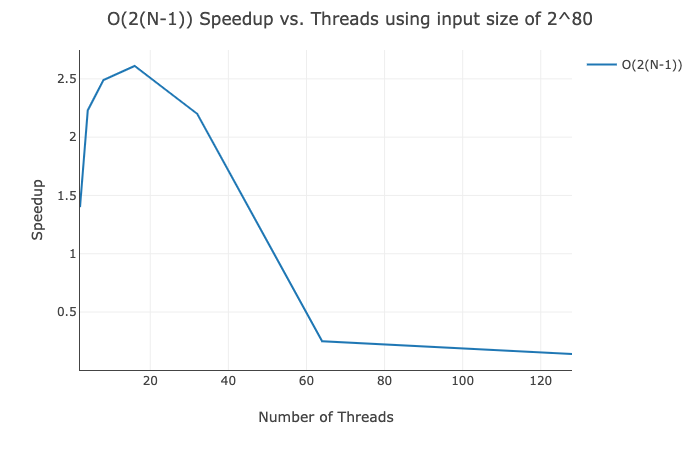
\includegraphics[scale=0.44]{plot}
		\end{figure}

	\section{Findings}
	Note: \(O(n-1)\): base, \(O(nlog(n))\): efficient serial, \(O(2(n-1))\): binary tree
	\begin{itemize}
		\item By using bit-wise operation rather than pow() function to get strides, the code gets better performance when input size is large.
		\item When serialized, binary tree method performs slightly worse than the efficient serial method. However, when parallelized, binary tree method gains speedup.
		\item For input size of 2\textasciicircum{}80, the binary tree method hits peak performance when using 16 threads.
	\end{itemize}

\end{document}